
When rvalue references were introduced in C++11 in support of move semantics, the traditional partitioning of expressions into lvalues and rvalues was no longer sufficient to describe all the C++11 language behaviors. The C++ standardization committee therefore redesigned the value category system based on three core and two composite categories (see Figure B.1). The core categories are: lvalue, prvalue (“pure rvalue”), and xvalue. The composite categories are: glvalue (“generalized lvalue,” which is the union of lvalue and xvalue) and rvalue (the union of xvalue and prvalue).

Note that all expressions are still either lvalues or rvalues, but the rvalues category is now further subdivided.

\begin{center}
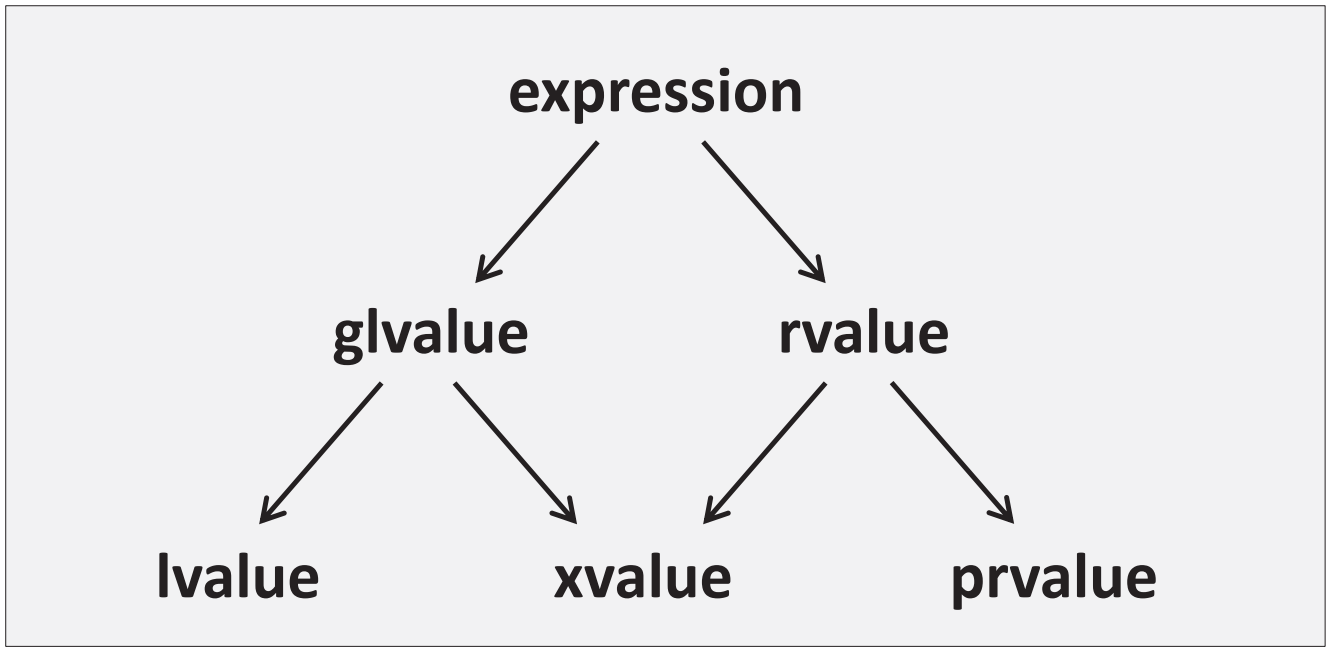
\includegraphics[width=0.8\textwidth]{content/Appendix/B/images/1.png} \\
Figure B.1. Value Categories since C++11
\end{center}

This C++11 categorization has remained in effect, but in C++17 the characterization of the categories were reformulated as follows:

\begin{itemize}
\item 
A glvalue is an expression whose evaluation determines the identity of an object, bit-field, or function (i.e., an entity that has storage).

\item 
A prvalue is an expression whose evaluation initializes an object or a bit-field, or computes the value of the operand of an operator.

\item 
An xvalue is a glvalue designating an object or bit-field whose resources can be reused (usually because it is about to “expire”—the “x” in xvalue originally came from “eXpiring value”).

\item 
An lvalue is a glvalue that is not an xvalue.

\item 
An rvalue is an expression that is either a prvalue or an xvalue.
\end{itemize}

Note that in C++17 (and to some extent, in C++11 and C++14), the glvalue vs. prvalue dichotomy is arguably more fundamental than the traditional lvalue vs. rvalue distinction.

Although this describes the characterization introduced in C++17, those descriptions also apply to C++11 and C++14 (the prior descriptions were equivalent but harder to reason about).

Except for bit fields, glvalues produce entities with an address. That address may be that of a subobject of a larger enclosing object. In the case of a base class subobject, the type of the glvalue (expression) is called its static type, and the type of the most derived object that base class is part of is called the dynamic type of the glvalue. If the glvalue does not produce a base class subobject, its static and dynamic types are identical (i.e., the type of the expression).

Examples of lvalues are:

\begin{itemize}
\item 
Expressions that designate variables or functions

\item 
Applications of the built-in unary * operator (“pointer indirection”)

\item 
An expression that is just a string literal

\item 
A call to a function with a return type that is an lvalue reference
\end{itemize}

Examples of prvalues are:

\begin{itemize}
\item 
Expressions that consist of a literal that is not a string literal or a user-defined literal

\begin{tcolorbox}[colback=webgreen!5!white,colframe=webgreen!75!black]
\hspace*{0.75cm}User-defined literals can lead to lvalues or rvalues, depending on the return type of the associated literal operator.
\end{tcolorbox}

\item 
Applications of the built-in unary \& operator (i.e., taking the address of an expression)

\item 
Applications of built-in arithmetic operators

\item 
A call to a function with a return type that is not a reference type

\item 
Lambda expressions
\end{itemize}

Examples of xvalues are:

\begin{itemize}
\item 
A call to a function with a return type that is an rvalue reference to an object type (e.g., std::move())

\item 
A cast to an rvalue reference to an object type
\end{itemize}

Note that rvalue references to function types produce lvalues, not xvalues.

It’s worth emphasizing that glvalues, prvalues, xvalues, and so on, are expressions, and not values

\begin{tcolorbox}[colback=webgreen!5!white,colframe=webgreen!75!black]
\hspace*{0.75cm}Which unfortunately means that these terms are misnomers.
\end{tcolorbox}

or entities. For example, a variable is not an lvalue even though an expression denoting a variable is an lvalue:

\begin{lstlisting}[style=styleCXX]
int x = 3; // x here is a variable, not an lvalue. 3 is a prvalue initializing
		  // the variable x.
int y = x; // x here is an lvalue. The evaluation of that lvalue expression does not
		  // produce the value 3, but a designation of an object containing the value 3.
		  // That lvalue is then then converted to a prvalue, which is what initializes y.
\end{lstlisting}

\subsubsubsection{B.2.1\hspace{0.2cm}Temporary Materialization}

We previously mentioned that lvalues often undergo an lvalue-to-rvalue conversion

\begin{tcolorbox}[colback=webgreen!5!white,colframe=webgreen!75!black]
\hspace*{0.75cm}In the world of C++11 value categories, the phrase glvalue-to-prvalue conversion would be more accurate, but the traditional term remains more common.
\end{tcolorbox}

because prvalues are the kinds of expressions that initialize objects (or provide the operands for most built-in operators).

In C++17, there is a dual to this conversion, known as temporary materialization (but it could just as well have been called “prvalue-to-xvalue conversion”): Any time a prvalue validly appears where a glvalue (which includes the xvalue case) is expected, a temporary object is created and initialized with the prvalue (recall that prvalues are primarily “initializing values”), and the prvalue is replaced by an xvalue designating the temporary. For example:

Because f() in this example has a reference parameter, it expects a glvalue argument. However, the expression 3 is a prvalue. The “temporary materialization” rule therefore kicks in, and the expression 3 is “converted” to an xvalue designating a temporary object initialized with the value 3.

More generally, a temporary is materialized to be initialized with a prvalue in the following situations:

\begin{itemize}
\item 
A prvalue is bound to a reference (e.g., that call f(3) above).

\item 
A member of a class prvalue is accessed.

\item 
An array prvalue is subscripted.

\item 
An array prvalue is converted to a pointer to its first element (i.e., array decay).

\item 
A prvalue appears in a braced initializer list that, for some type X, initializes an object of type std::initializer\_list<X>.

\item 
The sizeof or typeid operator is applied to a prvalue.

\item 
A prvalue is the top-level expression in a statement of the form “expr;” or an expression is cast to void.
\end{itemize}

Thus, in C++17, the object initialized by a prvalue is always determined by the context, and, as a result, temporaries are created only when they are really needed. Prior to C++17, prvalues (particularly of class type) always implied a temporary. Copies of those temporaries could optionally be elided later on, but a compiler still had to enforce most semantics constraints of the copy operation (e.g., a copy constructor may need to be callable). The following example shows a consequence of the C++17 revision of the rules:

\begin{lstlisting}[style=styleCXX]
class N {
	public:
	N();
	N(N const&) = delete; // this class is neither copyable ...
	N(N&&) = delete; // ... nor movable
};

N make_N() {
	return N{}; // Always creates a conceptual temporary prior to C++17.
} 				// In C++17, no temporary is created at this point.

auto n = make_N(); // ERROR prior to C++17 because the prvalue needs a
				// conceptual copy. OK since C++17, because n is
				// initialized directly from the prvalue.
\end{lstlisting}

Prior to C++17, the prvalue Nfg produced a temporary of type N, but compilers were allowed to elide copies and moves of that temporary (which they always did, in practice). In this case, that means that the temporary result of calling make\_N() can be constructed directly in the storage of n; no copy or move operation is needed. Unfortunately, pre-C++17 compilers still have to check that a copy or move operation could be made, and in this example that is not possible because the copy constructor of N is deleted (and no move constructor is generated). Hence, C++11 and C++14 compilers must issue an error for this example.

With C++17 the prvalue N itself does not produce a temporary. Instead, it initializes an object determined by the context: In our example, that object is the one denoted by n. No copy or move operation is ever considered (this is not an optimization, but a language guarantee) and therefore the code is valid C++17.

We conclude with an example that shows a variety of value category situations:

\begin{lstlisting}[style=styleCXX]
class X {
};

X v;
X const c;

void f(X const&); // accepts an expression of any value category
void f(X&&); // accepts prvalues and xvalues only but is a better match
			// for those than the previous declaration

f(v); // passes a modifiable lvalue to the first f()
f(c); // passes a nonmodifiable lvalue to the first f()
f(X()); // passes a prvalue (since C++17 materialized as xvalue) to the 2nd f()
f(std::move(v)); // passes an xvalue to the second f()
\end{lstlisting}









